\documentclass[1p]{elsarticle_modified}
%\bibliographystyle{elsarticle-num}

%\usepackage[colorlinks]{hyperref}
%\usepackage{abbrmath_seonhwa} %\Abb, \Ascr, \Acal ,\Abf, \Afrak
\usepackage{amsfonts}
\usepackage{amssymb}
\usepackage{amsmath}
\usepackage{amsthm}
\usepackage{scalefnt}
\usepackage{amsbsy}
\usepackage{kotex}
\usepackage{caption}
\usepackage{subfig}
\usepackage{color}
\usepackage{graphicx}
\usepackage{xcolor} %% white, black, red, green, blue, cyan, magenta, yellow
\usepackage{float}
\usepackage{setspace}
\usepackage{hyperref}

\usepackage{tikz}
\usetikzlibrary{arrows}

\usepackage{multirow}
\usepackage{array} % fixed length table
\usepackage{hhline}

%%%%%%%%%%%%%%%%%%%%%
\makeatletter
\renewcommand*\env@matrix[1][\arraystretch]{%
	\edef\arraystretch{#1}%
	\hskip -\arraycolsep
	\let\@ifnextchar\new@ifnextchar
	\array{*\c@MaxMatrixCols c}}
\makeatother %https://tex.stackexchange.com/questions/14071/how-can-i-increase-the-line-spacing-in-a-matrix
%%%%%%%%%%%%%%%

\usepackage[normalem]{ulem}

\newcommand{\msout}[1]{\ifmmode\text{\sout{\ensuremath{#1}}}\else\sout{#1}\fi}
%SOURCE: \msout is \stkout macro in https://tex.stackexchange.com/questions/20609/strikeout-in-math-mode

\newcommand{\cancel}[1]{
	\ifmmode
	{\color{red}\msout{#1}}
	\else
	{\color{red}\sout{#1}}
	\fi
}

\newcommand{\add}[1]{
	{\color{blue}\uwave{#1}}
}

\newcommand{\replace}[2]{
	\ifmmode
	{\color{red}\msout{#1}}{\color{blue}\uwave{#2}}
	\else
	{\color{red}\sout{#1}}{\color{blue}\uwave{#2}}
	\fi
}

\newcommand{\Sol}{\mathcal{S}} %segment
\newcommand{\D}{D} %diagram
\newcommand{\A}{\mathcal{A}} %arc


%%%%%%%%%%%%%%%%%%%%%%%%%%%%%5 test

\def\sl{\operatorname{\textup{SL}}(2,\Cbb)}
\def\psl{\operatorname{\textup{PSL}}(2,\Cbb)}
\def\quan{\mkern 1mu \triangleright \mkern 1mu}

\theoremstyle{definition}
\newtheorem{thm}{Theorem}[section]
\newtheorem{prop}[thm]{Proposition}
\newtheorem{lem}[thm]{Lemma}
\newtheorem{ques}[thm]{Question}
\newtheorem{cor}[thm]{Corollary}
\newtheorem{defn}[thm]{Definition}
\newtheorem{exam}[thm]{Example}
\newtheorem{rmk}[thm]{Remark}
\newtheorem{alg}[thm]{Algorithm}

\newcommand{\I}{\sqrt{-1}}
\begin{document}

%\begin{frontmatter}
%
%\title{Boundary parabolic representations of knots up to 8 crossings}
%
%%% Group authors per affiliation:
%\author{Yunhi Cho} 
%\address{Department of Mathematics, University of Seoul, Seoul, Korea}
%\ead{yhcho@uos.ac.kr}
%
%
%\author{Seonhwa Kim} %\fnref{s_kim}}
%\address{Center for Geometry and Physics, Institute for Basic Science, Pohang, 37673, Korea}
%\ead{ryeona17@ibs.re.kr}
%
%\author{Hyuk Kim}
%\address{Department of Mathematical Sciences, Seoul National University, Seoul 08826, Korea}
%\ead{hyukkim@snu.ac.kr}
%
%\author{Seokbeom Yoon}
%\address{Department of Mathematical Sciences, Seoul National University, Seoul, 08826,  Korea}
%\ead{sbyoon15@snu.ac.kr}
%
%\begin{abstract}
%We find all boundary parabolic representation of knots up to 8 crossings.
%
%\end{abstract}
%\begin{keyword}
%    \MSC[2010] 57M25 
%\end{keyword}
%
%\end{frontmatter}

%\linenumbers
%\tableofcontents
%
\newcommand\colored[1]{\textcolor{white}{\rule[-0.35ex]{0.8em}{1.4ex}}\kern-0.8em\color{red} #1}%
%\newcommand\colored[1]{\textcolor{white}{ #1}\kern-2.17ex	\textcolor{white}{ #1}\kern-1.81ex	\textcolor{white}{ #1}\kern-2.15ex\color{red}#1	}

{\Large $\underline{9_{29}~(K9a_{31})}$}

\setlength{\tabcolsep}{10pt}
\renewcommand{\arraystretch}{1.6}
\vspace{1cm}\begin{tabular}{m{100pt}>{\centering\arraybackslash}m{274pt}}
\multirow{5}{120pt}{
	\centering
	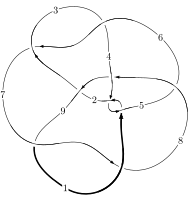
\includegraphics[width=112pt]{../../../GIT/diagram.site/Diagrams/png/64_9_29.png}\\
\ \ \ A knot diagram\footnotemark}&
\allowdisplaybreaks
\textbf{Linearized knot diagam} \\
\cline{2-2}
 &
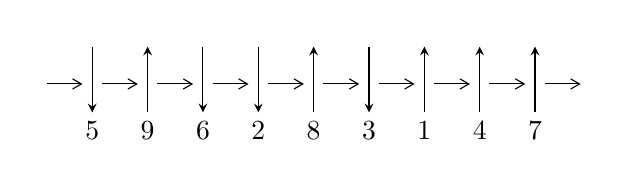
\begin{tikzpicture}[x=20pt, y=17pt]
	% nodes
	\node (C0) at (0, 0) {};
	\node (C1) at (1, 0) {};
	\node (C1U) at (1, +1) {};
	\node (C1D) at (1, -1) {5};

	\node (C2) at (2, 0) {};
	\node (C2U) at (2, +1) {};
	\node (C2D) at (2, -1) {9};

	\node (C3) at (3, 0) {};
	\node (C3U) at (3, +1) {};
	\node (C3D) at (3, -1) {6};

	\node (C4) at (4, 0) {};
	\node (C4U) at (4, +1) {};
	\node (C4D) at (4, -1) {2};

	\node (C5) at (5, 0) {};
	\node (C5U) at (5, +1) {};
	\node (C5D) at (5, -1) {8};

	\node (C6) at (6, 0) {};
	\node (C6U) at (6, +1) {};
	\node (C6D) at (6, -1) {3};

	\node (C7) at (7, 0) {};
	\node (C7U) at (7, +1) {};
	\node (C7D) at (7, -1) {1};

	\node (C8) at (8, 0) {};
	\node (C8U) at (8, +1) {};
	\node (C8D) at (8, -1) {4};

	\node (C9) at (9, 0) {};
	\node (C9U) at (9, +1) {};
	\node (C9D) at (9, -1) {7};
	\node (C10) at (10, 0) {};

	% arrows
	\draw[->,>={angle 60}]
	(C0) edge (C1) (C1) edge (C2) (C2) edge (C3) (C3) edge (C4) (C4) edge (C5) (C5) edge (C6) (C6) edge (C7) (C7) edge (C8) (C8) edge (C9) (C9) edge (C10) ;	\draw[->,>=stealth]
	(C1U) edge (C1D) (C2D) edge (C2U) (C3U) edge (C3D) (C4U) edge (C4D) (C5D) edge (C5U) (C6U) edge (C6D) (C7D) edge (C7U) (C8D) edge (C8U) (C9D) edge (C9U) ;
	\end{tikzpicture} \\
\hhline{~~} \\& 
\textbf{Solving Sequence} \\ \cline{2-2} 
 &
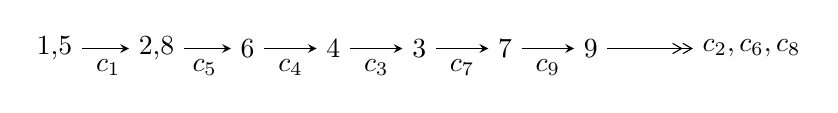
\begin{tikzpicture}[x=31pt, y=7pt]
	% node
	\node (A0) at (-1/8, 0) {1,5};
	\node (A1) at (17/16, 0) {2,8};
	\node (A2) at (17/8, 0) {6};
	\node (A3) at (25/8, 0) {4};
	\node (A4) at (33/8, 0) {3};
	\node (A5) at (41/8, 0) {7};
	\node (A6) at (49/8, 0) {9};
	\node (C1) at (1/2, -1) {$c_{1}$};
	\node (C2) at (13/8, -1) {$c_{5}$};
	\node (C3) at (21/8, -1) {$c_{4}$};
	\node (C4) at (29/8, -1) {$c_{3}$};
	\node (C5) at (37/8, -1) {$c_{7}$};
	\node (C6) at (45/8, -1) {$c_{9}$};
	\node (A7) at (8, 0) {$c_{2},c_{6},c_{8}$};

	% edge
	\draw[->,>=stealth]	
	(A0) edge (A1) (A1) edge (A2) (A2) edge (A3) (A3) edge (A4) (A4) edge (A5) (A5) edge (A6) ;
	\draw[->>,>={angle 60}]	
	(A6) edge (A7);
\end{tikzpicture} \\ 

\end{tabular} \\

\footnotetext{
The image of knot diagram is generated by the software ``\textbf{Draw programme}" developed by Andrew Bartholomew(\url{http://www.layer8.co.uk/maths/draw/index.htm\#Running-draw}), where we modified some parts for our purpose(\url{https://github.com/CATsTAILs/LinksPainter}).
}\phantom \\ \newline 
\centering \textbf{Ideals for irreducible components\footnotemark of $X_{\text{par}}$} 
 
\begin{align*}
I^u_{1}&=\langle 
u^9-2 u^8+6 u^7-9 u^6+13 u^5-19 u^4+14 u^3-12 u^2+4 b+7 u-1,\\
\phantom{I^u_{1}}&\phantom{= \langle  }3 u^9-6 u^8+18 u^7-31 u^6+47 u^5-65 u^4+58 u^3-56 u^2+8 a+29 u-11,\\
\phantom{I^u_{1}}&\phantom{= \langle  }u^{10}- u^9+4 u^8-7 u^7+8 u^6-14 u^5+11 u^4-10 u^3+7 u^2-2 u-1\rangle \\
I^u_{2}&=\langle 
3488 u^{15}+8516 u^{14}+\cdots+887 b+5098,\;5348 u^{15}+12394 u^{14}+\cdots+887 a+7607,\\
\phantom{I^u_{2}}&\phantom{= \langle  }u^{16}+3 u^{15}+\cdots+2 u+1\rangle \\
I^u_{3}&=\langle 
b-1,\;2 a-1,\;u-1\rangle \\
\\
\end{align*}
\raggedright * 3 irreducible components of $\dim_{\mathbb{C}}=0$, with total 27 representations.\\
\footnotetext{All coefficients of polynomials are rational numbers. But the coefficients are sometimes approximated in decimal forms when there is not enough margin.}
\newpage
\renewcommand{\arraystretch}{1}
\centering \section*{I. $I^u_{1}= \langle u^9-2 u^8+\cdots+4 b-1,\;3 u^9-6 u^8+\cdots+8 a-11,\;u^{10}- u^9+\cdots-2 u-1 \rangle$}
\flushleft \textbf{(i) Arc colorings}\\
\begin{tabular}{m{7pt} m{180pt} m{7pt} m{180pt} }
\flushright $a_{1}=$&$\begin{pmatrix}1\\0\end{pmatrix}$ \\
\flushright $a_{5}=$&$\begin{pmatrix}0\\u\end{pmatrix}$ \\
\flushright $a_{2}=$&$\begin{pmatrix}1\\u^2\end{pmatrix}$ \\
\flushright $a_{8}=$&$\begin{pmatrix}-\frac{3}{8} u^9+\frac{3}{4} u^8+\cdots-\frac{29}{8} u+\frac{11}{8}\\-\frac{1}{4} u^9+\frac{1}{2} u^8+\cdots-\frac{7}{4} u+\frac{1}{4}\end{pmatrix}$ \\
\flushright $a_{6}=$&$\begin{pmatrix}\frac{1}{16} u^9-\frac{1}{8} u^8+\cdots+\frac{31}{16} u-\frac{17}{16}\\\frac{1}{8} u^9-\frac{1}{4} u^8+\cdots+\frac{15}{8} u-\frac{1}{8}\end{pmatrix}$ \\
\flushright $a_{4}=$&$\begin{pmatrix}u\\u^3+u\end{pmatrix}$ \\
\flushright $a_{3}=$&$\begin{pmatrix}\frac{1}{16} u^9-\frac{1}{8} u^8+\cdots+\frac{31}{16} u-\frac{1}{16}\\\frac{1}{8} u^9-\frac{1}{4} u^8+\cdots+\frac{7}{8} u-\frac{1}{8}\end{pmatrix}$ \\
\flushright $a_{7}=$&$\begin{pmatrix}-\frac{1}{8} u^9+\frac{1}{4} u^8+\cdots-\frac{15}{8} u+\frac{9}{8}\\-\frac{1}{4} u^9+\frac{1}{2} u^8+\cdots-\frac{7}{4} u+\frac{1}{4}\end{pmatrix}$ \\
\flushright $a_{9}=$&$\begin{pmatrix}-\frac{7}{8} u^9+\frac{3}{4} u^8+\cdots-\frac{17}{8} u+\frac{15}{8}\\\frac{3}{4} u^9-\frac{1}{2} u^8+\cdots-\frac{7}{4} u+\frac{1}{4}\end{pmatrix}$\\ \flushright $a_{9}=$&$\begin{pmatrix}-\frac{7}{8} u^9+\frac{3}{4} u^8+\cdots-\frac{17}{8} u+\frac{15}{8}\\\frac{3}{4} u^9-\frac{1}{2} u^8+\cdots-\frac{7}{4} u+\frac{1}{4}\end{pmatrix}$\\&\end{tabular}
\flushleft \textbf{(ii) Obstruction class $= -1$}\\~\\
\flushleft \textbf{(iii) Cusp Shapes $= -\frac{37}{16} u^9-\frac{3}{8} u^8-\frac{55}{8} u^7+\frac{145}{16} u^6-\frac{41}{16} u^5+\frac{351}{16} u^4-\frac{35}{8} u^3+\frac{19}{2} u^2-\frac{219}{16} u+\frac{85}{16}$}\\~\\
\newpage\renewcommand{\arraystretch}{1}
\flushleft \textbf{(iv) u-Polynomials at the component}\newline \\
\begin{tabular}{m{50pt}|m{274pt}}
Crossings & \hspace{64pt}u-Polynomials at each crossing \\
\hline $$\begin{aligned}c_{1},c_{3},c_{4}\\c_{6}\end{aligned}$$&$\begin{aligned}
&u^{10}+u^9+4 u^8+7 u^7+8 u^6+14 u^5+11 u^4+10 u^3+7 u^2+2 u-1
\end{aligned}$\\
\hline $$\begin{aligned}c_{2},c_{5}\end{aligned}$$&$\begin{aligned}
&2(2 u^{10}+3 u^9-4 u^8-8 u^7+9 u^6+7 u^5-5 u^4-2 u^3- u+1)
\end{aligned}$\\
\hline $$\begin{aligned}c_{7},c_{9}\end{aligned}$$&$\begin{aligned}
&u^{10}-4 u^8+u^7+5 u^6-3 u^5+12 u^4+18 u^3-7 u^2-11 u-4
\end{aligned}$\\
\hline $$\begin{aligned}c_{8}\end{aligned}$$&$\begin{aligned}
&u^{10}-3 u^9+3 u^8+8 u^7-7 u^6-30 u^5+80 u^4-60 u^3+41 u^2-30 u+8
\end{aligned}$\\
\hline
\end{tabular}\\~\\
\newpage\renewcommand{\arraystretch}{1}
\flushleft \textbf{(v) Riley Polynomials at the component}\newline \\
\begin{tabular}{m{50pt}|m{274pt}}
Crossings & \hspace{64pt}Riley Polynomials at each crossing \\
\hline $$\begin{aligned}c_{1},c_{3},c_{4}\\c_{6}\end{aligned}$$&$\begin{aligned}
&y^{10}+7 y^9+\cdots-18 y+1
\end{aligned}$\\
\hline $$\begin{aligned}c_{2},c_{5}\end{aligned}$$&$\begin{aligned}
&4(4 y^{10}-25 y^9+\cdots- y+1)
\end{aligned}$\\
\hline $$\begin{aligned}c_{7},c_{9}\end{aligned}$$&$\begin{aligned}
&y^{10}-8 y^9+\cdots-65 y+16
\end{aligned}$\\
\hline $$\begin{aligned}c_{8}\end{aligned}$$&$\begin{aligned}
&y^{10}-3 y^9+\cdots-244 y+64
\end{aligned}$\\
\hline
\end{tabular}\\~\\
\newpage\flushleft \textbf{(vi) Complex Volumes and Cusp Shapes}
$$\begin{array}{c|c|c}  
\text{Solutions to }I^u_{1}& \I (\text{vol} + \sqrt{-1}CS) & \text{Cusp shape}\\
 \hline 
\begin{aligned}
u &= \phantom{-}0.642531 + 0.377867 I \\
a &= \phantom{-}0.425417 + 0.618053 I \\
b &= -0.388235 + 0.305929 I\end{aligned}
 & -1.18006 - 1.03831 I & -4.73685 + 3.71172 I \\ \hline\begin{aligned}
u &= \phantom{-}0.642531 - 0.377867 I \\
a &= \phantom{-}0.425417 - 0.618053 I \\
b &= -0.388235 - 0.305929 I\end{aligned}
 & -1.18006 + 1.03831 I & -4.73685 - 3.71172 I \\ \hline\begin{aligned}
u &= -0.296868 + 1.222110 I \\
a &= -0.265428 + 0.874553 I \\
b &= \phantom{-}0.310628 + 1.327070 I\end{aligned}
 & \phantom{-}4.73127 + 5.96240 I & \phantom{-}6.55763 - 6.45237 I \\ \hline\begin{aligned}
u &= -0.296868 - 1.222110 I \\
a &= -0.265428 - 0.874553 I \\
b &= \phantom{-}0.310628 - 1.327070 I\end{aligned}
 & \phantom{-}4.73127 - 5.96240 I & \phantom{-}6.55763 + 6.45237 I \\ \hline\begin{aligned}
u &= \phantom{-}0.090479 + 1.266340 I \\
a &= -0.180352 - 0.660546 I \\
b &= \phantom{-}1.72873 - 0.67558 I\end{aligned}
 & \phantom{-}8.92450 - 2.36890 I & \phantom{-}11.53570 + 2.96432 I \\ \hline\begin{aligned}
u &= \phantom{-}0.090479 - 1.266340 I \\
a &= -0.180352 + 0.660546 I \\
b &= \phantom{-}1.72873 + 0.67558 I\end{aligned}
 & \phantom{-}8.92450 + 2.36890 I & \phantom{-}11.53570 - 2.96432 I \\ \hline\begin{aligned}
u &= \phantom{-}1.36651\phantom{ +0.000000I} \\
a &= -0.570064\phantom{ +0.000000I} \\
b &= -1.16409\phantom{ +0.000000I}\end{aligned}
 & \phantom{-}0.587104\phantom{ +0.000000I} & \phantom{-}12.3230\phantom{ +0.000000I} \\ \hline\begin{aligned}
u &= -0.50395 + 1.40837 I \\
a &= \phantom{-}0.204381 - 1.196050 I \\
b &= -1.50564 - 0.50027 I\end{aligned}
 & \phantom{-}10.4508 + 12.2059 I & \phantom{-}7.05765 - 6.58910 I \\ \hline\begin{aligned}
u &= -0.50395 - 1.40837 I \\
a &= \phantom{-}0.204381 + 1.196050 I \\
b &= -1.50564 + 0.50027 I\end{aligned}
 & \phantom{-}10.4508 - 12.2059 I & \phantom{-}7.05765 + 6.58910 I \\ \hline\begin{aligned}
u &= -0.230893\phantom{ +0.000000I} \\
a &= \phantom{-}2.70203\phantom{ +0.000000I} \\
b &= \phantom{-}0.873110\phantom{ +0.000000I}\end{aligned}
 & \phantom{-}1.26306\phantom{ +0.000000I} & \phantom{-}9.09880\phantom{ +0.000000I}\\
 \hline 
 \end{array}$$\newpage\newpage\renewcommand{\arraystretch}{1}
\centering \section*{II. $I^u_{2}= \langle 3488 u^{15}+8516 u^{14}+\cdots+887 b+5098,\;5348 u^{15}+12394 u^{14}+\cdots+887 a+7607,\;u^{16}+3 u^{15}+\cdots+2 u+1 \rangle$}
\flushleft \textbf{(i) Arc colorings}\\
\begin{tabular}{m{7pt} m{180pt} m{7pt} m{180pt} }
\flushright $a_{1}=$&$\begin{pmatrix}1\\0\end{pmatrix}$ \\
\flushright $a_{5}=$&$\begin{pmatrix}0\\u\end{pmatrix}$ \\
\flushright $a_{2}=$&$\begin{pmatrix}1\\u^2\end{pmatrix}$ \\
\flushright $a_{8}=$&$\begin{pmatrix}-6.02931 u^{15}-13.9729 u^{14}+\cdots-2.86809 u-8.57610\\-3.93236 u^{15}-9.60090 u^{14}+\cdots-2.30440 u-5.74746\end{pmatrix}$ \\
\flushright $a_{6}=$&$\begin{pmatrix}7.33709 u^{15}+15.6888 u^{14}+\cdots+5.98309 u+15.1251\\3.02593 u^{15}+7.05299 u^{14}+\cdots+3.38331 u+5.16347\end{pmatrix}$ \\
\flushright $a_{4}=$&$\begin{pmatrix}u\\u^3+u\end{pmatrix}$ \\
\flushright $a_{3}=$&$\begin{pmatrix}-4.12176 u^{15}-9.11838 u^{14}+\cdots+4.54791 u-3.85457\\-0.676437 u^{15}-1.99098 u^{14}+\cdots+2.04397 u-0.525366\end{pmatrix}$ \\
\flushright $a_{7}=$&$\begin{pmatrix}-2.09696 u^{15}-4.37204 u^{14}+\cdots-0.563698 u-2.82864\\-3.93236 u^{15}-9.60090 u^{14}+\cdots-2.30440 u-5.74746\end{pmatrix}$ \\
\flushright $a_{9}=$&$\begin{pmatrix}-4.00451 u^{15}-9.22661 u^{14}+\cdots-1.97971 u-5.55017\\-1.15896 u^{15}-3.23788 u^{14}+\cdots-0.784667 u-1.39346\end{pmatrix}$\\ \flushright $a_{9}=$&$\begin{pmatrix}-4.00451 u^{15}-9.22661 u^{14}+\cdots-1.97971 u-5.55017\\-1.15896 u^{15}-3.23788 u^{14}+\cdots-0.784667 u-1.39346\end{pmatrix}$\\&\end{tabular}
\flushleft \textbf{(ii) Obstruction class $= -1$}\\~\\
\flushleft \textbf{(iii) Cusp Shapes $= \frac{14664}{887} u^{15}+\frac{36136}{887} u^{14}+\cdots+\frac{12068}{887} u+\frac{27426}{887}$}\\~\\
\newpage\renewcommand{\arraystretch}{1}
\flushleft \textbf{(iv) u-Polynomials at the component}\newline \\
\begin{tabular}{m{50pt}|m{274pt}}
Crossings & \hspace{64pt}u-Polynomials at each crossing \\
\hline $$\begin{aligned}c_{1},c_{3},c_{4}\\c_{6}\end{aligned}$$&$\begin{aligned}
&u^{16}-3 u^{15}+\cdots-2 u+1
\end{aligned}$\\
\hline $$\begin{aligned}c_{2},c_{5}\end{aligned}$$&$\begin{aligned}
&u^{16}- u^{15}+\cdots+136 u+47
\end{aligned}$\\
\hline $$\begin{aligned}c_{7},c_{9}\end{aligned}$$&$\begin{aligned}
&(u^8+u^7-3 u^6-2 u^5+3 u^4+2 u-1)^2
\end{aligned}$\\
\hline $$\begin{aligned}c_{8}\end{aligned}$$&$\begin{aligned}
&(u^8+u^7- u^6-2 u^5+u^4+2 u^3-2 u-1)^2
\end{aligned}$\\
\hline
\end{tabular}\\~\\
\newpage\renewcommand{\arraystretch}{1}
\flushleft \textbf{(v) Riley Polynomials at the component}\newline \\
\begin{tabular}{m{50pt}|m{274pt}}
Crossings & \hspace{64pt}Riley Polynomials at each crossing \\
\hline $$\begin{aligned}c_{1},c_{3},c_{4}\\c_{6}\end{aligned}$$&$\begin{aligned}
&y^{16}+11 y^{15}+\cdots+20 y^2+1
\end{aligned}$\\
\hline $$\begin{aligned}c_{2},c_{5}\end{aligned}$$&$\begin{aligned}
&y^{16}-9 y^{15}+\cdots-13044 y+2209
\end{aligned}$\\
\hline $$\begin{aligned}c_{7},c_{9}\end{aligned}$$&$\begin{aligned}
&(y^8-7 y^7+19 y^6-22 y^5+3 y^4+14 y^3-6 y^2-4 y+1)^2
\end{aligned}$\\
\hline $$\begin{aligned}c_{8}\end{aligned}$$&$\begin{aligned}
&(y^8-3 y^7+7 y^6-10 y^5+11 y^4-10 y^3+6 y^2-4 y+1)^2
\end{aligned}$\\
\hline
\end{tabular}\\~\\
\newpage\flushleft \textbf{(vi) Complex Volumes and Cusp Shapes}
$$\begin{array}{c|c|c}  
\text{Solutions to }I^u_{2}& \I (\text{vol} + \sqrt{-1}CS) & \text{Cusp shape}\\
 \hline 
\begin{aligned}
u &= -0.181988 + 1.048500 I \\
a &= \phantom{-}1.25894 + 1.17937 I \\
b &= \phantom{-}0.463640\phantom{ +0.000000I}\end{aligned}
 & \phantom{-}4.13490\phantom{ +0.000000I} & \phantom{-}7.89446 + 0. I\phantom{ +0.000000I} \\ \hline\begin{aligned}
u &= -0.181988 - 1.048500 I \\
a &= \phantom{-}1.25894 - 1.17937 I \\
b &= \phantom{-}0.463640\phantom{ +0.000000I}\end{aligned}
 & \phantom{-}4.13490\phantom{ +0.000000I} & \phantom{-}7.89446 + 0. I\phantom{ +0.000000I} \\ \hline\begin{aligned}
u &= -1.142130 + 0.104845 I \\
a &= -0.895766 - 0.516597 I \\
b &= -1.334530 - 0.318930 I\end{aligned}
 & \phantom{-}5.66955 + 6.44354 I & \phantom{-}5.42845 - 5.29417 I \\ \hline\begin{aligned}
u &= -1.142130 - 0.104845 I \\
a &= -0.895766 + 0.516597 I \\
b &= -1.334530 + 0.318930 I\end{aligned}
 & \phantom{-}5.66955 - 6.44354 I & \phantom{-}5.42845 + 5.29417 I \\ \hline\begin{aligned}
u &= \phantom{-}0.309237 + 1.112330 I \\
a &= \phantom{-}0.034672 - 0.683601 I \\
b &= \phantom{-}0.108090 - 0.747508 I\end{aligned}
 & \phantom{-}1.13045 - 2.57849 I & \phantom{-}0.27708 + 3.56796 I \\ \hline\begin{aligned}
u &= \phantom{-}0.309237 - 1.112330 I \\
a &= \phantom{-}0.034672 + 0.683601 I \\
b &= \phantom{-}0.108090 + 0.747508 I\end{aligned}
 & \phantom{-}1.13045 + 2.57849 I & \phantom{-}0.27708 - 3.56796 I \\ \hline\begin{aligned}
u &= -0.072810 + 1.153150 I \\
a &= -1.02661 + 1.10040 I \\
b &= \phantom{-}1.180120 + 0.268597 I\end{aligned}
 & \phantom{-}4.33052 + 1.13123 I & \phantom{-}3.41522 - 0.51079 I \\ \hline\begin{aligned}
u &= -0.072810 - 1.153150 I \\
a &= -1.02661 - 1.10040 I \\
b &= \phantom{-}1.180120 - 0.268597 I\end{aligned}
 & \phantom{-}4.33052 - 1.13123 I & \phantom{-}3.41522 + 0.51079 I \\ \hline\begin{aligned}
u &= -0.597255 + 0.026660 I \\
a &= \phantom{-}1.20070 - 1.29659 I \\
b &= \phantom{-}0.108090 - 0.747508 I\end{aligned}
 & \phantom{-}1.13045 - 2.57849 I & \phantom{-}0.27708 + 3.56796 I \\ \hline\begin{aligned}
u &= -0.597255 - 0.026660 I \\
a &= \phantom{-}1.20070 + 1.29659 I \\
b &= \phantom{-}0.108090 + 0.747508 I\end{aligned}
 & \phantom{-}1.13045 + 2.57849 I & \phantom{-}0.27708 - 3.56796 I\\
 \hline 
 \end{array}$$\newpage$$\begin{array}{c|c|c}  
\text{Solutions to }I^u_{2}& \I (\text{vol} + \sqrt{-1}CS) & \text{Cusp shape}\\
 \hline 
\begin{aligned}
u &= \phantom{-}0.50715 + 1.45748 I \\
a &= \phantom{-}0.219942 + 0.896459 I \\
b &= -1.334530 + 0.318930 I\end{aligned}
 & \phantom{-}5.66955 - 6.44354 I & \phantom{-}5.42845 + 5.29417 I \\ \hline\begin{aligned}
u &= \phantom{-}0.50715 - 1.45748 I \\
a &= \phantom{-}0.219942 - 0.896459 I \\
b &= -1.334530 - 0.318930 I\end{aligned}
 & \phantom{-}5.66955 + 6.44354 I & \phantom{-}5.42845 - 5.29417 I \\ \hline\begin{aligned}
u &= -0.60300 + 1.44597 I \\
a &= -0.091711 - 0.669730 I \\
b &= -1.37100\phantom{ +0.000000I}\end{aligned}
 & \phantom{-}9.79260\phantom{ +0.000000I} & \phantom{-}9.86404 + 0. I\phantom{ +0.000000I} \\ \hline\begin{aligned}
u &= -0.60300 - 1.44597 I \\
a &= -0.091711 + 0.669730 I \\
b &= -1.37100\phantom{ +0.000000I}\end{aligned}
 & \phantom{-}9.79260\phantom{ +0.000000I} & \phantom{-}9.86404 + 0. I\phantom{ +0.000000I} \\ \hline\begin{aligned}
u &= \phantom{-}0.280801 + 0.318917 I \\
a &= \phantom{-}3.29984 - 0.74872 I \\
b &= \phantom{-}1.180120 - 0.268597 I\end{aligned}
 & \phantom{-}4.33052 - 1.13123 I & \phantom{-}3.41522 + 0.51079 I \\ \hline\begin{aligned}
u &= \phantom{-}0.280801 - 0.318917 I \\
a &= \phantom{-}3.29984 + 0.74872 I \\
b &= \phantom{-}1.180120 + 0.268597 I\end{aligned}
 & \phantom{-}4.33052 + 1.13123 I & \phantom{-}3.41522 - 0.51079 I\\
 \hline 
 \end{array}$$\newpage\newpage\renewcommand{\arraystretch}{1}
\centering \section*{III. $I^u_{3}= \langle b-1,\;2 a-1,\;u-1 \rangle$}
\flushleft \textbf{(i) Arc colorings}\\
\begin{tabular}{m{7pt} m{180pt} m{7pt} m{180pt} }
\flushright $a_{1}=$&$\begin{pmatrix}1\\0\end{pmatrix}$ \\
\flushright $a_{5}=$&$\begin{pmatrix}0\\1\end{pmatrix}$ \\
\flushright $a_{2}=$&$\begin{pmatrix}1\\1\end{pmatrix}$ \\
\flushright $a_{8}=$&$\begin{pmatrix}0.5\\1\end{pmatrix}$ \\
\flushright $a_{6}=$&$\begin{pmatrix}0.25\\1.5\end{pmatrix}$ \\
\flushright $a_{4}=$&$\begin{pmatrix}1\\2\end{pmatrix}$ \\
\flushright $a_{3}=$&$\begin{pmatrix}0.75\\0.5\end{pmatrix}$ \\
\flushright $a_{7}=$&$\begin{pmatrix}-0.5\\1\end{pmatrix}$ \\
\flushright $a_{9}=$&$\begin{pmatrix}0.5\\1\end{pmatrix}$\\ \flushright $a_{9}=$&$\begin{pmatrix}0.5\\1\end{pmatrix}$\\&\end{tabular}
\flushleft \textbf{(ii) Obstruction class $= 1$}\\~\\
\flushleft \textbf{(iii) Cusp Shapes $= -2.25$}\\~\\
\newpage\renewcommand{\arraystretch}{1}
\flushleft \textbf{(iv) u-Polynomials at the component}\newline \\
\begin{tabular}{m{50pt}|m{274pt}}
Crossings & \hspace{64pt}u-Polynomials at each crossing \\
\hline $$\begin{aligned}c_{1},c_{3},c_{9}\end{aligned}$$&$\begin{aligned}
&u-1
\end{aligned}$\\
\hline $$\begin{aligned}c_{2}\end{aligned}$$&$\begin{aligned}
&2(2 u-1)
\end{aligned}$\\
\hline $$\begin{aligned}c_{4},c_{6},c_{7}\end{aligned}$$&$\begin{aligned}
&u+1
\end{aligned}$\\
\hline $$\begin{aligned}c_{5}\end{aligned}$$&$\begin{aligned}
&2(2 u+1)
\end{aligned}$\\
\hline $$\begin{aligned}c_{8}\end{aligned}$$&$\begin{aligned}
&u
\end{aligned}$\\
\hline
\end{tabular}\\~\\
\newpage\renewcommand{\arraystretch}{1}
\flushleft \textbf{(v) Riley Polynomials at the component}\newline \\
\begin{tabular}{m{50pt}|m{274pt}}
Crossings & \hspace{64pt}Riley Polynomials at each crossing \\
\hline $$\begin{aligned}c_{1},c_{3},c_{4}\\c_{6},c_{7},c_{9}\end{aligned}$$&$\begin{aligned}
&y-1
\end{aligned}$\\
\hline $$\begin{aligned}c_{2},c_{5}\end{aligned}$$&$\begin{aligned}
&4(4 y-1)
\end{aligned}$\\
\hline $$\begin{aligned}c_{8}\end{aligned}$$&$\begin{aligned}
&y
\end{aligned}$\\
\hline
\end{tabular}\\~\\
\newpage\flushleft \textbf{(vi) Complex Volumes and Cusp Shapes}
$$\begin{array}{c|c|c}  
\text{Solutions to }I^u_{3}& \I (\text{vol} + \sqrt{-1}CS) & \text{Cusp shape}\\
 \hline 
\begin{aligned}
u &= \phantom{-}1.00000\phantom{ +0.000000I} \\
a &= \phantom{-}0.500000\phantom{ +0.000000I} \\
b &= \phantom{-}1.00000\phantom{ +0.000000I}\end{aligned}
 & \phantom{-0.000000 } 0 & -2.25000\phantom{ +0.000000I}\\
 \hline 
 \end{array}$$\newpage
\newpage\renewcommand{\arraystretch}{1}
\centering \section*{ IV. u-Polynomials}
\begin{tabular}{m{50pt}|m{274pt}}
Crossings & \hspace{64pt}u-Polynomials at each crossing \\
\hline $$\begin{aligned}c_{1},c_{3}\end{aligned}$$&$\begin{aligned}
&(u-1)(u^{10}+u^9+\cdots+2 u-1)\\
&\cdot(u^{16}-3 u^{15}+\cdots-2 u+1)
\end{aligned}$\\
\hline $$\begin{aligned}c_{2}\end{aligned}$$&$\begin{aligned}
&4(2 u-1)(2 u^{10}+3 u^9-4 u^8-8 u^7+9 u^6+7 u^5-5 u^4-2 u^3- u+1)\\
&\cdot(u^{16}- u^{15}+\cdots+136 u+47)
\end{aligned}$\\
\hline $$\begin{aligned}c_{4},c_{6}\end{aligned}$$&$\begin{aligned}
&(u+1)(u^{10}+u^9+\cdots+2 u-1)\\
&\cdot(u^{16}-3 u^{15}+\cdots-2 u+1)
\end{aligned}$\\
\hline $$\begin{aligned}c_{5}\end{aligned}$$&$\begin{aligned}
&4(2 u+1)(2 u^{10}+3 u^9-4 u^8-8 u^7+9 u^6+7 u^5-5 u^4-2 u^3- u+1)\\
&\cdot(u^{16}- u^{15}+\cdots+136 u+47)
\end{aligned}$\\
\hline $$\begin{aligned}c_{7}\end{aligned}$$&$\begin{aligned}
&(u+1)(u^8+u^7-3 u^6-2 u^5+3 u^4+2 u-1)^2\\
&\cdot(u^{10}-4 u^8+u^7+5 u^6-3 u^5+12 u^4+18 u^3-7 u^2-11 u-4)
\end{aligned}$\\
\hline $$\begin{aligned}c_{8}\end{aligned}$$&$\begin{aligned}
&u(u^8+u^7- u^6-2 u^5+u^4+2 u^3-2 u-1)^2\\
&\cdot(u^{10}-3 u^9+3 u^8+8 u^7-7 u^6-30 u^5+80 u^4-60 u^3+41 u^2-30 u+8)
\end{aligned}$\\
\hline $$\begin{aligned}c_{9}\end{aligned}$$&$\begin{aligned}
&(u-1)(u^8+u^7-3 u^6-2 u^5+3 u^4+2 u-1)^2\\
&\cdot(u^{10}-4 u^8+u^7+5 u^6-3 u^5+12 u^4+18 u^3-7 u^2-11 u-4)
\end{aligned}$\\
\hline
\end{tabular}\newpage\renewcommand{\arraystretch}{1}
\centering \section*{ V. Riley Polynomials}
\begin{tabular}{m{50pt}|m{274pt}}
Crossings & \hspace{64pt}Riley Polynomials at each crossing \\
\hline $$\begin{aligned}c_{1},c_{3},c_{4}\\c_{6}\end{aligned}$$&$\begin{aligned}
&(y-1)(y^{10}+7 y^9+\cdots-18 y+1)(y^{16}+11 y^{15}+\cdots+20 y^2+1)
\end{aligned}$\\
\hline $$\begin{aligned}c_{2},c_{5}\end{aligned}$$&$\begin{aligned}
&16(4 y-1)(4 y^{10}-25 y^9+\cdots- y+1)\\
&\cdot(y^{16}-9 y^{15}+\cdots-13044 y+2209)
\end{aligned}$\\
\hline $$\begin{aligned}c_{7},c_{9}\end{aligned}$$&$\begin{aligned}
&(y-1)(y^8-7 y^7+19 y^6-22 y^5+3 y^4+14 y^3-6 y^2-4 y+1)^2\\
&\cdot(y^{10}-8 y^9+\cdots-65 y+16)
\end{aligned}$\\
\hline $$\begin{aligned}c_{8}\end{aligned}$$&$\begin{aligned}
&y(y^8-3 y^7+7 y^6-10 y^5+11 y^4-10 y^3+6 y^2-4 y+1)^2\\
&\cdot(y^{10}-3 y^9+\cdots-244 y+64)
\end{aligned}$\\
\hline
\end{tabular}
\vskip 2pc
\end{document}